%!TEX root = thesis.tex
\section{Low Fields}

Similar to the previous chapter, we will start this one by defining what is meant by low applied magnetic fields. As we saw before, we are dealing with polycrystalline ferromagnetic bodies which, in general, are highly non-linear and they show a hysteretical behavior. In order to analyze the case of low fields in a meaningful way that, in addition behaves less complex mathematically, we took first the assumption of our material being soft magnetic, taking away the hysteretic behavior. The next step, will be to tackle the nonlinearity by analyzing the two different cases: high fields and low fields. In both of these cases, we linearize our curve. In the high fields case to be a constant (saturation) and in this case to be a linear relation of the following structure.

\begin{equation}
\textbf{M}(\textbf{r}) = \chi_m \textbf{H}(\textbf{r})
\end{equation}

Although we already used this variable name to describe the nonlinear curve we will be consistent with the convention of using for low fields $\chi_m$ as a constant parameter. 

\subsection{The Demagnetization Tensor}

Now that there is a relation that tells us how the body magnetizes for low fields, we can combine it to our integral equation (that basically calculates how the magnetic field looks like for a magnetized body). The solution to the equation is the real physical state that our body achieves.

\begin{equation}
\frac{1}{\chi_m}\textbf{M}(\textbf{r}) = -\mathcal{N}(\textbf{r},\textbf{M}(\textbf{r}))  + \textbf{H}_\text{app}
\end{equation}

Since there's a linear relation between the total H-Field and the magnetization we can either solve the above equation to $\textbf{M}$ or to $\textbf{H}$. In our case it will be convenient to solve it to $\textbf{M}$.\\

Although there is no general closed solution to the above equation, it can be proved (see Appendix \ref{s:LinearityIntegralEquation}) that the magnetization $\textbf{M}(\textbf{r})$ is linear towards the the applied field $\textbf{H}_\text{app}$. From that it follows that the demagnetization field  $\textbf{H}_d(\textbf{r})$ and the total H-Field $\textbf{H}(\textbf{r})$ also are. The main theorems of linear algebra allow us to describe any linear relation through a matrix multiplication. We can therefore define a new matrix $\Psi(\textbf{r})$:

\begin{equation}
\textbf{M}(\textbf{r}) = \Psi(\textbf{r})\textbf{H}_\text{app}
\end{equation}

from the definition of the demagnetization field it follows:

\begin{equation}
\textbf{H}_d(\textbf{r}) = \left(\frac{1}{\chi_m}\Psi(\textbf{r})-I\right)\textbf{H}_\text{app}
\end{equation}

and the total field:

\begin{equation}
\textbf{H}(\textbf{r}) = \frac{1}{\chi_m}\Psi(\textbf{r})\textbf{H}_\text{app}
\end{equation}

Our integral equation now becomes:

\begin{equation}
\frac{1}{\chi_m}\Psi(\textbf{r}) = -\mathcal{N}(\textbf{r},\Psi(\textbf{r}))  + I
\end{equation}

and its solution, the matrix function $\Psi(\textbf{r})$.\\

The problem here, is that we have no clear definition of what the demagnetization factor for low fields may be. We define it then, to be consistent to the high fields case: We use the a set of three linearly independent applied fields and construct the matrices $H_\text{app}$, $M(\textbf{r})$, $H(\textbf{r})$ and $H_d(\textbf{r})$ such that:

\begin{subequations}
\begin{equation}
H(\textbf{r}) := [\textbf{H}_1(\textbf{r}), \textbf{H}_2(\textbf{r}), \textbf{H}_3(\textbf{r})]
\end{equation}
\begin{equation}
M(\textbf{r}) := [\textbf{M}_1(\textbf{r}), \textbf{M}_2(\textbf{r}), \textbf{M}_3(\textbf{r})]
\end{equation}
\begin{equation}
H_\text{app} := [\textbf{H}_{\text{app},1}, \textbf{H}_{\text{app},2}, \textbf{H}_{\text{app},3}]
\end{equation}
\end{subequations}

We now define the demagnetization tensor for low fields in the following way:

\begin{equation}
N(\textbf{r}) := -H_d(\textbf{r})\,M(\textbf{r})^{-1}
\end{equation}

and through simplification we get\footnote{a detailed derivation can be found in Appendix \ref{s:DemagPsi}}:

\begin{equation}
N(\textbf{r}) = \Psi(\textbf{r})^{-1} - \frac{1}{\chi_m}I
\end{equation}

\subsection{Calculation through simulation}

Like in the case of high fields, our basic calculation will be the simulation in COMSOL. For this part, the same models, meshes and assumptions were used, with the difference that here, a linear model was used instead of a non-linear one that can be saturated. The reason for this is to be consistent with the fact that we are dealing with low fields, which makes the model act linearly. \\

We will use the same method as before calculating the magnetization for three linear independent applied fields and calculating the demagnetization factor with the following relation:

\begin{equation}
 N(\textbf{r}) =  H_d(\textbf{r})   M(\textbf{r})  ^{-1}
\end{equation}

which is correct and consistent to our definition for low fields.

\subsubsection{Averaged Values}

Since, again, we are dealing with averaged values, it is very important to leave clear mathematically what we are doing while taking any assumption. In the case of high fields (saturated case), the magnetization of the body is assumed to be constant. One could write it in the following fashion:

\begin{equation}
\langle N(\textbf{r}) \rangle = \langle H_d(\textbf{r}) \rangle  M_s ^{-1} = \langle H_d(\textbf{r}) \rangle \langle M(\textbf{r}) \rangle ^{-1}
\end{equation}

This basically says, that the averaged demagnetization matrix can be calculated as a product of two averaged matrices. Since the magnetization matrix is anyways constant, averaging has no effect on it. However in the low field case, the averaged demagnetization tensor is not the product of the averaged applied field matrix and the inverse of the averaged magnetization matrix. Since

\begin{equation}
\langle N(\textbf{r}) \rangle = \langle \Psi({\textbf{r})}^{-1}\rangle - \frac{1}{\chi_m}I
\end{equation}

and

\begin{equation}
 \langle H_d(\textbf{r}) \rangle \langle M(\textbf{r}) \rangle ^{-1} = \langle \Psi({\textbf{r})}\rangle^{-1} - \frac{1}{\chi_m}I
\end{equation}

However, we will make the assumption of $\langle\Psi(\textbf{r})\rangle^{-1} \approx \langle\Psi(\textbf{r})^{-1}\rangle$ in order to perform our calculations over simulations in the same fashion as it has been explained before, thus using the following relation:

\begin{equation}
\langle N(\textbf{r}) \rangle \approx \langle H_d(\textbf{r}) \rangle \langle M(\textbf{r}) \rangle ^{-1}
\end{equation}

An deep analysis and further research on this topic will be need in order to assess the correctness of this assumption. The mathematical properties of the demagnetization matrix depending on the properties of $\Psi(\textbf{r})$ and $\langle\Psi(\textbf{r})\rangle$ will.

\subsubsection{Results}

Analogously to the high field case, the results of the simulations for the full magnetic, thin coated and half coated are presented in Figure \ref{fig:DemagLow}. 

\begin{figure}[ht]
	\centering
  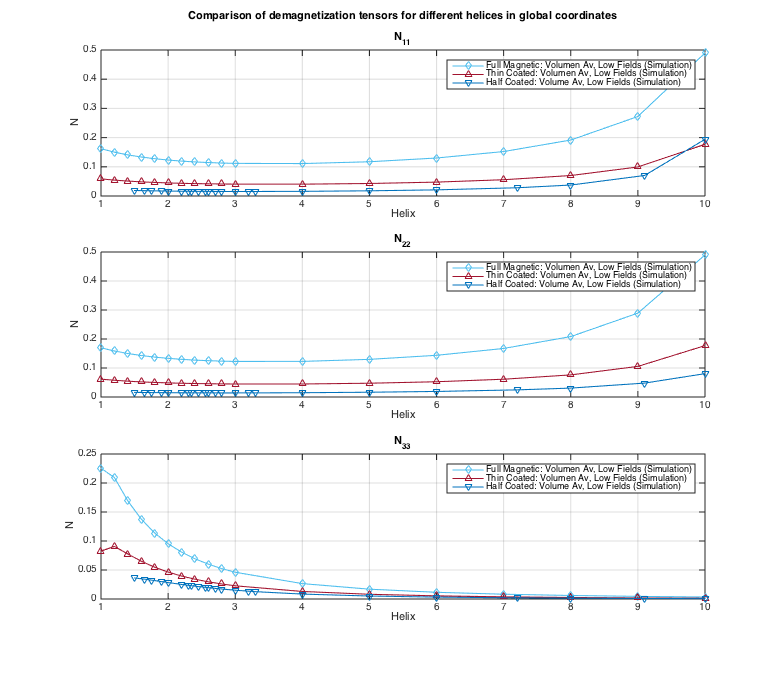
\includegraphics[width=1\textwidth]{Pictures/DemagFactors_Comparison_Low.png}
	\caption{Diagonal values of demagnetization matrices of helical soft-magnetic helices with high permeability at low fields}
	\label{fig:DemagLow}
\end{figure}

The misalignment angles are, again, shown in Figure \ref{fig:MisalignmentAngles_Low} compared to the experimental data.

\begin{figure}[ht]
	\centering
  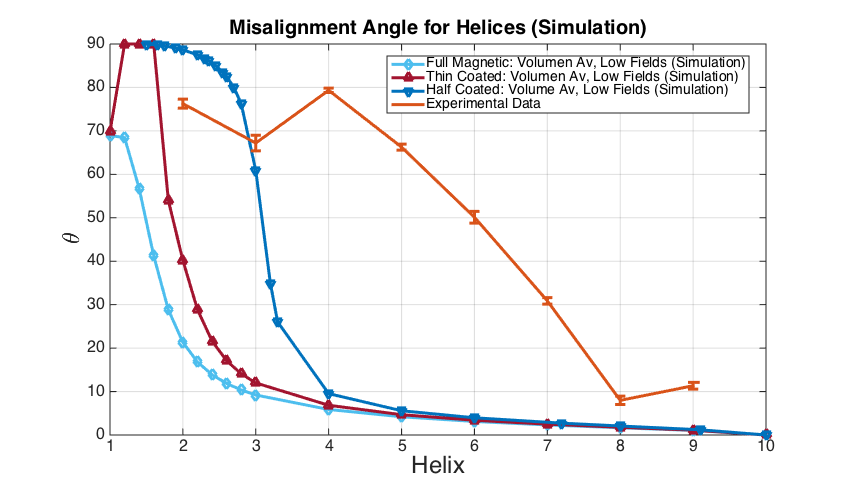
\includegraphics[width=1\textwidth]{Pictures/MisalignmentAngles_Low.png}
	\caption{Misalignment angles of helical soft-magnetic helices with high permeability at low fields}
	\label{fig:MisalignmentAngles_Low}
\end{figure}

In Figure \ref{fig:DemagLow} we clearly see the the same trends on all curves. As expected we a see a very similar behavior between both radial axes (directions 1 and 2), on all three curves. The reason for this is the small influence of the top and bottom end of each helix (it is not an infinitely long helix) which accounts for the differences. 
The results are easier to interpret with the fact that the magnetization of a helix for low fields follows in each point the shape and direction of the helix (See Figure \ref{fig:MagnetLow}\\

In directions 1 and 2 (radial directions) we see that the curves start at a certain level, diminish and then grow again. This means in other words, that the helices magnetize harder for lower helix index in radial direction, then easier and finally hard again. As it was mentioned before, the magnetization points along the shape of the helix. Since the helix is coiled, and we're dealing with the total magnetization, the coiling creates a cancellation of magnetization for most of the helix. When the helix has a more elongated form (not fully elongated) this cancellation effect goes away and the helix magnetizes therefore easier along the specific direction. When the helix is very elongated the helix is almost aligned with the third axes. Since the helix is very slim, it is very difficult to magnetize in radial directions.\\

In the case of direction 3 we see a constant drop from the coiled helices to the more elongated helices. The reason for this is that, when the helix is coiled, it is hard to magnetize in the third direction, which is the direction perpendicular to the helix's shape line. When the helix elongates, the helix's shape line aligns more and more with the third direction, which makes every time more easy to magnetize, the more the helix elongates, therefore the drop in the demagnetization factor.\\

The discrepancies between the three types of helix fillings (full, thin shell and half-coated) is due to the fact that the body magnetizes easier along the thin film. In the case of thin shell, the helix magnetizes easier along the wall, but the fact of it being round accounts also for cancellations in the field (depending on the direction of the applied field). In the case of the half-coated helices, the cancellation doesn't appear. The coiling of the helix but also the local orientation combined with the type of filling create complex interactions, which account for the shifting of the curves. The plots are evidence, that the coiling of the helix is the predominant factor when it comes to the qualitative, main magnetic behavior of the helix, and not the type of filling of it. \\

Figure \ref{fig:MisalignmentAngles_Low} we see the misalignment angles compared to the experimentally measured misalignment angles. Again, we captured the trend of the misalignment angle: For low coiled helices, the misalignment angle tends towards a perpendicular alignment with the applied field, whereas, as expected, for more elongated helices the alignment correspond to the direction of the applied field, behaving more like a compass needle.\\

\begin{figure}[ht]
	\centering
  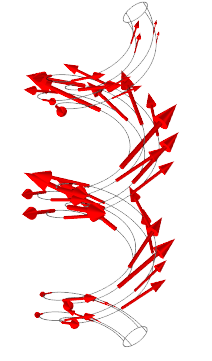
\includegraphics[width=0.2\textwidth]{Pictures/MagnetLow.png}
	\caption{Graphical representation of magnetization of a ferromagnetic helix in low fields. The arrows (red) represent the magnetization vectors in different points along the helix}
	\label{fig:MagnetLow}
\end{figure}


\subsection{Analytical Calculation}

Contrary to the high field case, where the demagnetization factor is only a surface integral matrix, for the low field case, one has to solve the surface integral matrix equation:

\begin{equation}
\frac{1}{\chi_m}\Psi(\textbf{r}) = -\mathcal{N}(\textbf{r},\Psi(\textbf{r}))  + I
\end{equation}

the demagnetization factor is then:

\begin{equation}
N(\textbf{r}) = \Psi(\textbf{r})^{-1} - \frac{1}{\chi_m}I
\end{equation}

From the problem formulation, the solution seems to be uncomplicated. However this was one of the biggest challenges throughout this report. The first approach was to approximate our integral equation by a line integral, by assuming that the integrand doesn't change much from the center to the edges (since the wire is very thin).This turned our surface integral equation into a so called Fredholm integral equation with a linear integral operator in it (see Appendix) for which there exist literature that tackles the problem of solving it numerically (see  \cite{Allahviranloo2011}, \cite{Babolian2004}, \cite{DeBonis2008}, \cite{Hameed2011}, \cite{Jafarian2012}, \cite{Karimi2015}, \cite{Maleknejad2005},\cite{Rashidinia2007}, \cite{Ray2013}, \cite{Saeed2008}). After unsuccessful implementation of various methods (mainly because of the numerical complexity) we developed the following algorithm to solve it.

\subsubsection{Solving Algorithm}

In this subsection we'll explain the numerical algorithm used to solve the Matrix integral equation shown above. The principle lies in the idea of approximating each component of the matrix $\Psi(s)$ by another function. The choice of these approximations were Fourier series and Legendre polynomials.\\

Lets write our matrix $\Psi(s)$ as an approximation $\hat{\Psi}(s)$ of some basic functions. For the component $i,j$ we have:

\begin{subequations}
\begin{equation}
\hat{\Psi}_{i,j}(s)  = c_{i,j}^1f_1(s) + c_{i,j}^Nf_N(s) + ... + c_{i,j}^Nf_N(s) = 
\end{equation}
\begin{equation}
\underbrace{ \left[ 
\begin{array} {c}
c_{i,j}^1 \\
c_{i,j}^2 \\
\vdots \\
c_{i,j}^N \\
\end{array}\right]}_{=:c_{i,j}} \cdot \underbrace{\left[ 
\begin{array} {c}
f_1(s) \\
f_2(s) \\
\vdots \\
f_N(s) \\
\end{array}\right]}_{=:f(s)}
\end{equation}
\end{subequations}

We can then write the matrix in the following way:

\begin{equation}
\hat{\Psi}(s) = \underbrace{ \left(\begin{array}{ccc}
f(s)^T & 0 \dots &  \dots 0 \\
0 \dots & f(s)^T & \dots 0 \\
0 \dots & \dots 0 & f(s)^T\\
\end{array} \right)}_{=:F(s)}\underbrace{ \left(\begin{array}{ccc}
c_{1,1} & c_{1,2} & c_{1,3}   \\
c_{2,1} & c_{2,2} & c_{2,3}   \\
c_{3,1} & c_{3,2} & c_{3,3}   \\
\end{array} \right)}_{=:C}
\end{equation}

If we plug our approximation in the integral equation we get:
\begin{subequations}
\begin{equation}
\frac{1}{\chi_m}\hat{\Psi}(s) = - \mathcal{N}(\hat{\Psi}(s)) + I
\end{equation}
\begin{equation}
\frac{1}{\chi_m}F(s)C = - \mathcal{N}(F(s))C + I
\end{equation}
\begin{equation}
\frac{1}{\chi_m}(F(s) + \mathcal{N}(F(s)))C  = I
\end{equation}
\begin{equation}
(F(s) + \mathcal{N}(F(s)))C  = \chi_mI
\end{equation}
\end{subequations}

The matrix $(F(s) + \mathcal{N}(F(s)))$ is a $3\times 3N$ Matrix. So in order to make it square we evaluate it at $N$ points of $s$. We become then:


\begin{equation}
\underbrace{\left[ \begin{array}{c}
(F(s_1) + \mathcal{N}(F(s_1)))   \\
(F(s_2) + \mathcal{N}(F(s_2)))  \\
\vdots \\
(F(s_N) + \mathcal{N}(F(s_3)))  \\
\end{array} \right]}_{:=A} C = 
\underbrace{\left[ \begin{array}{c}
\chi_mI  \\
\chi_mI  \\
\vdots \\
\chi_mI  \\
\end{array} \right]}_{:=B}
\end{equation}

And finally:

\begin{equation}
C = A^{-1}B
\end{equation}


This means that we reduced our integral equation to a linear system, where we have to calculate $9N^2$ integrals.\\

Unfortunately the results obtained by this algorithm were not successful (mainly due to no convergence and singularities in the results) and the task of solving the integral equation was left for further research. \\

The methods of solving problems in magnetostatics is a topic that has been researched for many decades. We will leave further research try to approach the problem using the methods used until now. For more information, refer to:\cite{Babic2000}, \cite{Canova2001}, \cite{Hafla2005}, \cite{Hafla2006a}, \cite{Hafla2006}, \cite{Hafla2006b}, \cite{Han1994}, \cite{Le-van2015}, \cite{Maleknejad2005}, \cite{Nicolazzi2005}, \cite{Nicolet1994}, \cite{Sertel2002}, \cite{Shahi2009} and \cite{VandeWiele2008}.
